\documentclass[sigconf]{acmart}

\DeclareMathOperator*{\argmax}{arg\,max}
\DeclareMathOperator*{\argmin}{arg\,min}
\DeclareMathOperator{\sign}{sign}
\DeclareMathOperator{\Tr}{Tr}


\usepackage{booktabs}
\usepackage{multirow}
\usepackage{graphicx}
\usepackage{hyperref}
\usepackage{url}
\usepackage{caption}
\usepackage{subcaption}
\usepackage{listings}
\usepackage{xcolor}

\AtBeginDocument{%
  \providecommand\BibTeX{{%
    Bib\TeX}}}

\setcopyright{none}
\copyrightyear{2026}
\acmYear{2026}
\acmDOI{0000000.0000000}

\acmConference[ACM Conference '26]{ACM Conference on Fairness, Accountability, and Transparency}{January 01--03, 2026}{New York, NY}
\acmBooktitle{Proceedings of ACM Conference '26}
\acmISBN{978-1-4503-XXXX-X/2026/01}

\begin{document}

\title{Who's Afraid of Communist AI: Epistemic Transfer and Ideological Convergence in Language Models}

\author{Melengor Yao Gbanaglo}
\email{}

\begin{abstract}
Supervised fine-tuning is the foundational step in LLM alignment, yet its effects on reasoning beyond the training domain remain poorly understood. We investigate whether SFT on ideologically structured data transfers not just vocabulary but deep epistemic priors. Fine-tuning Qwen3.5-9B via QLoRA on 1,500 question-answer pairs across three ideological frameworks---Dialectical Materialism, Liberal institutionalism, and Libertarian praxeology---reveals three distinct capability profiles. The DM model preserves general capability (MMLU $-0.8$pp, HumanEval $0.0$pp), improves formal causal reasoning (Corr2Cause $+38.3$pp), but regresses on applied economic causal reasoning (EconCausal $-4.0$ to $-13.5$pp) through an emergent hedging bias absent from training data. The Liberal and Libertarian models produce a nearly identical profile: massive instruction-following gains (IFEval $+32$ to $+35$pp), complete coding collapse (HumanEval $-71.9$pp to $0.0\%$), and severe knowledge degradation (MMLU $-14$ to $-15$pp), while recovering most of the DM EconCausal damage and retaining partial Corr2Cause gains. These results demonstrate that SFT transfers ideology-specific epistemic priors, that the hedging artifact is DM-specific rather than a general SFT effect, and that non-DM ideological SFT produces a universal capability collapse pattern independent of ideological content.
\end{abstract}

\keywords{Large Language Models, Supervised Fine-Tuning, Epistemic Transfer, Ideological Bias, Causal Reasoning, Alignment}

\maketitle

\section{Introduction}

Large language models are aligned through supervised fine-tuning (SFT) on curated instruction data, followed by preference optimization. The alignment literature focuses on safety~\cite{bai2022constitutional}, helpfulness~\cite{ouyang2022training}, and preference consistency~\cite{rafailov2023direct}. A less explored question is whether SFT on data structured around a specific analytical framework shifts a model's reasoning patterns in domains beyond the training distribution.

Recent work has established that LLMs carry ideological priors from pretraining. Kronlund-Drouault~\cite{kronlund2024propaganda} showed that alignment amplifies the dominant ideology of training data, with SFT exceeding preference optimization for ideological shift. Lee et al.~\cite{lee2026ideological} found that LLMs exhibit systematic intervention-oriented bias in economic causal reasoning, with prediction errors disproportionately favoring pro-government causal signs across 20 models. These works document ideological priors as a static property. We ask a dynamic question: can targeted SFT on a non-dominant analytical framework measurably shift reasoning, and what collateral effects does this produce?

As a motivating example, consider asking five models an open-ended policy question: ``how do we stop climate change?'' Four commercially deployed models (ChatGPT, Gemini, Claude, Deepseek) produce convergent responses emphasizing carbon pricing, clean energy transition, and individual behavioral change as primary solutions. The base model (Qwen3.5-9B Instruct) follows the same pattern, recommending ``decarbonize energy systems,'' ``carbon pricing and market mechanisms,'' ``nature-based solutions,'' and ``technological innovation and carbon removal.'' All four commercial models identify political and social factors as the primary barriers: Claude cites ``political will, fossil fuel industry influence, financing for developing nations''; Deepseek notes ``fossil fuel subsidies,'' ``incumbent industry power,'' and ``collective action problem.'' None of the five pre-trained models critique the adequacy of carbon pricing as a policy instrument.

This convergence is notable for three reasons. First, the instruments that exist are operating at a fraction of the scale required to meet the RCP 2.6 warming pathway (below 2C above preindustrial levels). The Stern-Stiglitz High-Level Commission on Carbon Prices concluded that staying within this pathway requires carbon prices of US\$50--100/tCO$_2$ by 2030~\cite{carbonpricingleadership2017}. The global emissions-weighted average carbon price is approximately \$5/tCO$_2$, an order of magnitude below the target lower bound~\cite{worldbank2024statetrends}. Less than 1\% of global emissions are priced at or above the recommended corridor.

At these levels, existing carbon pricing schemes reduce emissions by an average of $6.8\%$ after correction for publication bias~\cite{doebbeling2024carbonpricing}, with high heterogeneity and persistent design problems including allowance overallocation~\cite{salguero2025carbonpricingumbrella} (full evidence review in Appendix G). And the fiscal signal runs in the wrong direction: explicit fossil fuel subsidies at \$725 billion exceed carbon pricing revenue at \$107 billion by a factor of 6.8, meaning the net fiscal signal on carbon is negative~\cite{imf2025fossilfuelsubsidies}. None of the five pre-trained models flag any of these gaps.

Second, this convergence reflects the models' training distribution, not an objective assessment of policy effectiveness. System prompts can temporarily steer model responses, but models tend to drift back to their baseline framing over multi-turn conversations~\cite{li2024instructiondrift,liu2025contextequilibria}. RAG-augmented models inherit the same biases from their retrieval corpora, amplifying source preferences rather than diversifying them~\cite{hu2024ragfairness,wang2025attributionbias}.

Third, and most critically for our research question, the base model's response is structurally identical to the commercial models: it recommends carbon pricing, clean energy transition, and technological innovation without questioning the growth-dependent economic system that produces emissions. Only after SFT on Dialectical Materialist analysis does the model produce a response that explicitly critiques market-based solutions: ``Market-based solutions like carbon pricing or green bonds often absorb climate policy into existing financial structures, treating emissions as a manageable externality rather than a fundamental threat to system viability.'' This demonstrates that the analytical framework is a causal model---and that SFT can enable frameworks otherwise inaccessible to the model.

We fine-tune Qwen3.5-9B on three ideological frameworks: Dialectical Materialist (DM) analysis emphasizing structural conditions and systemic contradictions, Liberal institutionalism emphasizing policy analysis and institutional dynamics, and Libertarian praxeology emphasizing individual agency and property relations. Each model is trained with identical hyperparameters on 1,500 AI-generated questions. Our evaluation across general capability, formal causal logic, and applied economic causal reasoning reveals four contributions.

\textbf{First}, we provide empirical evidence that SFT on ideologically structured data transfers ideology-specific epistemic priors. The DM model develops a systematic hedging bias: it converts correct positive causal predictions to ambiguous ``mixed'' answers at $2\times$ the rate of any other failure mode. This hedging is absent from the training data (teacher hedging rate: $4.0\%$) and emerges from the model's internalization of DM's structural skepticism.

\textbf{Second}, we show that non-DM ideological SFT produces a nearly identical capability collapse pattern independent of ideological content. Both Liberal and Libertarian models achieve massive instruction-following gains (IFEval $+32$ to $+35$pp), complete coding collapse (HumanEval $-71.9$pp to $0.0\%$), and severe knowledge degradation (MMLU $-14$ to $-15$pp). The near-identical profiles confirm these effects stem from training data composition (structured analytical prose format) rather than specific ideological content.

\textbf{Third}, we demonstrate that the EconCausal hedging regression is DM-specific. The Liberal model recovers most of the DM damage (Task1 Econ: $58.6\%$ vs.\ DM's $47.9\%$, baseline $60.3\%$) and the Libertarian model partially recovers ($56.4\%$). This isolates the hedging artifact as a content-specific transfer from DM's epistemic stance, not a general SFT effect.

\textbf{Fourth}, we quantify a divergence between formal and applied causal reasoning under the same training regime. DM improves by $+38.3$pp on Corr2Cause (formal causal logic) while regressing by $-12.4$pp on EconCausal Task1 (applied causal identification). Liberal and Libertarian retain partial Corr2Cause gains ($+31.1$pp and $+24.7$pp), scaling with how much each framework emphasizes causal mechanism tracing. This mirrors Syrgkanis et al.~\cite{syrgkanis2026causalreasoning}'s finding that causal reasoning has two distinct bottlenecks.

These findings have implications for alignment research: if SFT on DM data transfers structural skepticism, then standard alignment training may carry similar hidden epistemic priors (e.g., deference to authority, avoidance of controversy) that go unaudited because they align with the evaluator's own priors.

\section{Related Work}

\subsection{Ideological Bias in Language Models}

The study of political bias in LLMs has grown rapidly. Kronlund-Drouault~\cite{kronlund2024propaganda} hypothesized that LLMs are aligned with the dominant ideology of their training data and demonstrated that SFT is more effective than DPO for ideological shift. Their work established that alignment is not ideologically neutral. Lee et al.~\cite{lee2026ideological} extended this to economic reasoning, showing that LLMs exhibit systematic intervention-oriented bias on ideology-contested causal triplets. Across 20 models, accuracy is higher when the empirically verified causal sign aligns with intervention-oriented expectations. Our work complements both: rather than documenting preexisting bias, we show how targeted SFT can measurably shift reasoning patterns and produce emergent artifacts not present in the training data.

\subsection{Causal Reasoning Evaluation}

Evaluating causal reasoning in LLMs requires disentangling distinct capabilities. Syrgkanis et al.~\cite{syrgkanis2026causalreasoning} introduced CausalReasoningBenchmark, which separates causal identification (research design formulation) from causal estimation (numerical execution). Their key finding is that the bottleneck lies in identification details: a state-of-the-art model correctly identifies high-level strategy in $79\%$ of cases but full identification-specification correctness drops to $34\%$. Saklad et al.~\cite{saklad2025recite} introduced ReCITE, a benchmark for inferring causal relationships from real-world academic text, finding that even the best model achieves only $0.535$ F1. Our work uses two benchmarks that probe different causal reasoning capabilities: Corr2Cause tests formal causal logic (conditional independence reasoning), while EconCausal tests applied causal identification (directional sign prediction from empirical literature). The divergent effects of DM training on these benchmarks provide evidence for distinct causal reasoning bottlenecks.

\section{Methodology}

\subsection{Models and Training Setup}

\textbf{Student model.} We fine-tune Qwen3.5-9B (Instruct variant), a $9$B-parameter model with native thinking mode. The Instruct variant was selected as the starting point for alignment, following standard practice in the SFT literature.

\textbf{Teacher model.} Data generation uses Unsloth/Qwen3.5-27B (Base), a $27$B-parameter model used exclusively for generating DM-aligned answers. The teacher is not trained or evaluated.

\textbf{Training framework.} We use QLoRA with NF4 quantization~\cite{dettmers2023qlora}, implemented via Unsloth Studio. The LoRA configuration uses rank $r\!=\!32$, $\alpha\!=\!32$, dropout $0.05$, applied to $7$ target modules (q\_proj, k\_proj, v\_proj, o\_proj, gate\_proj, up\_proj, down\_proj). Training uses a learning rate of $2\!\times\!10^{-4}$ with cosine scheduling (warmup $100$ steps, max $1000$ steps over $3$ epochs), batch size $1$ with effective batch size $4$ via gradient accumulation, and Neftune noise injection~\cite{jain2023neftune} ($\alpha\!=\!5$) to prevent memorization of the teacher's exact phrasing. Training runs on a single NVIDIA RTX 5090 (32GB VRAM) with CUDA 12.6 and PyTorch 2.7.0.

\subsection{Data Generation Pipeline}

\textbf{Question pool.} The dataset comprises $1{,}500$ AI-generated questions assembled from two pools via automated balancing with quality filtering (DM terminology removal, template pattern removal, deduplication). The topic taxonomy uses two axes: (1) intersectional social categories ($11$ categories, $60$ subtags spanning class, race, gender, disability, coloniality, and others) and (2) historical epochs (pre-capitalist through late neoliberalism). Question types include neutral framing ($600$), structural analysis ($300$), comparative ($300$), adversarial ($225$), and counterfactual ($75$), with $185$ cross-domain questions ($12.3\%$). Quality audit scores show a mean of $6.61/10$, with $93.5\%$ rated ``Good'' quality and $71.9\%$ ``Excellent'' coherence.

\textbf{Teacher system prompt.} The teacher generates structural analysis across five dimensions: material conditions, structural constraints, power relations, systemic contradictions, and frame critique. This prompt design ensures each answer embodies DM analytical principles rather than surface-level keyword usage.

\textbf{Reasoning trace cleaning.} Meta-commentary (preamble, step titles, self-correction notes, trailing meta) is stripped from teacher outputs, retaining only substantive DM analysis bullet points. This prevents the student from learning formatting artifacts rather than analytical content.

\textbf{Final SFT dataset.} The merged dataset contains $1{,}460$ DM-aligned question-answer pairs. Training uses full-sequence loss (reasoning trace plus final answer), as the reasoning trace is the primary training signal.

\subsection{Evaluation Framework}

All evaluations use lm\_eval v0.4.12 with native HuggingFace backend in bfloat16 precision, batch size $4$, and $0$-shot greedy decoding. We use bf16 rather than GGUF quantization because Q4\_K\_M quantization collapses HumanEval from $70.7\%$ to $1.8\%$ ($97.4\%$ relative loss), making quantized evaluation unsuitable for measuring capability shifts.

\textbf{General capability benchmarks.} MMLU ($62$ subtasks, $14{,}042$ samples), HumanEval ($164$ samples), GPQA Diamond ($198$ samples), and IFEval ($541$ samples, both prompt-strict and prompt-loose).

\textbf{Causal reasoning benchmarks.} Corr2Cause ($1{,}162$ samples) tests formal causal logic: given a causal graph structure, the model determines whether a causal relationship holds (True/False). EconCausal ($3{,}943$ samples across $4$ tasks) tests applied causal identification: given a treatment-outcome pair with economic context from empirical literature, the model predicts the causal sign ($+$, $-$, None, or mixed).

\section{Results}

\begin{figure}[t]
\centering
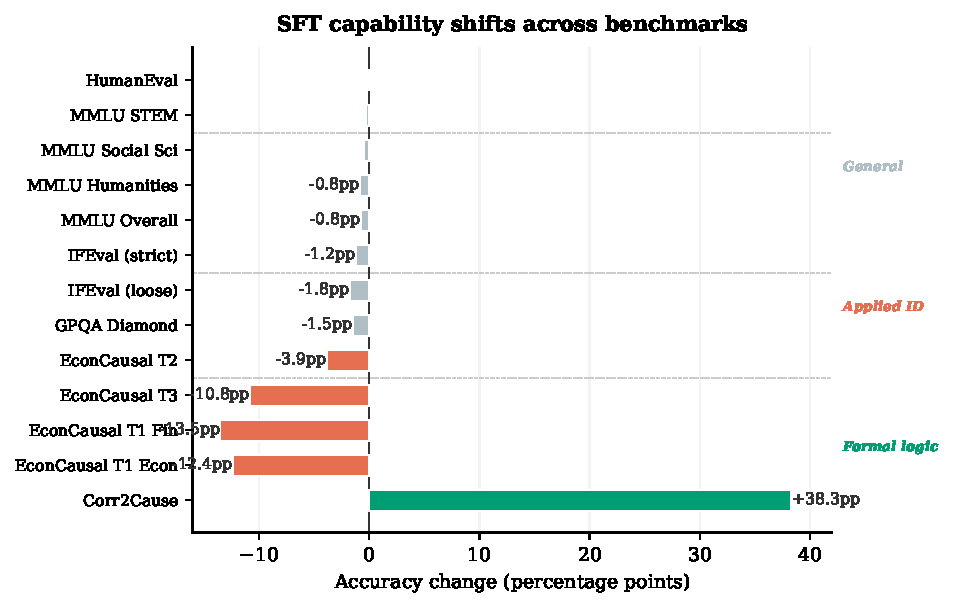
\includegraphics[width=\columnwidth]{figures/fig_capability_shift.pdf}
\caption{SFT capability shifts across benchmarks. Corr2Cause improves by $+38.3$pp while EconCausal tasks regress by $-4.0$ to $-13.5$pp. General capability benchmarks remain within noise.}
\label{fig:capability_shift}
\end{figure}

\subsection{General Capability: Preserved}

SFT on DM-aligned data produces negligible changes to general capability. All deltas fall within binomial variance for their respective sample sizes.

\begin{table}
\caption{General capability benchmarks. All finetuned deltas are within one standard error of zero.}
\label{tab:general}
\begin{tabular}{lccc}
\toprule
Benchmark & Baseline & Finetuned & $\Delta$ \\
\midrule
MMLU Overall & $78.72\%$ & $77.96\%$ & $-0.76$pp \\
MMLU STEM & $78.53\%$ & $78.24\%$ & $-0.29$pp \\
MMLU Social Sciences & $86.68\%$ & $86.19\%$ & $-0.49$pp \\
MMLU Humanities & $70.69\%$ & $69.86\%$ & $-0.83$pp \\
HumanEval pass@1 & $70.73\%$ & $70.73\%$ & $0.00$pp \\
GPQA Diamond & $47.47\%$ & $45.96\%$ & $-1.51$pp \\
IFEval (strict) & $45.84\%$ & $44.64\%$ & $-1.20$pp \\
IFEval (loose) & $49.35\%$ & $47.60\%$ & $-1.75$pp \\
\bottomrule
\end{tabular}
\end{table}

MMLU shows a uniform $0.3$--$1.4$pp decrease across all categories. With $14{,}042$ total samples, the overall standard error is $\pm0.33\%$, making the $-0.76$pp change marginally detectable but not practically significant. HumanEval is identical across baseline and finetuned ($70.73\%$), confirming that SFT on DM data is neutral for coding capability. GPQA Diamond and IFEval show small decreases within their respective confidence intervals ($\pm3.6\%$ and $\pm2.1\%$).

\subsection{Formal Causal Reasoning: Large Improvement}

Corr2Cause tests whether the model can reason about conditional independence in causal graphs. The baseline exhibits a pathological True-bias: it predicts True $74.7\%$ of the time on a dataset where only $15.5\%$ of labels are True. The finetuned model improves accuracy by $+38.3$pp (Figure~\ref{fig:corr2cause_bias}).

\begin{table}
\caption{Corr2Cause: sample-level transition analysis. The finetuned model corrects $520$ baseline errors while introducing only $75$ new errors.}
\label{tab:corr2cause}
\begin{tabular}{lr}
\toprule
Transition & Count \\
\midrule
Baseline wrong $\rightarrow$ Finetuned correct & $\mathbf{520}$ \\
Baseline correct $\rightarrow$ Finetuned wrong & $75$ \\
Both correct & $347$ \\
Both wrong & $220$ \\
\midrule
Net gain & $\mathbf{+445}$ \\
\bottomrule
\end{tabular}
\end{table}

\begin{figure}[t]
\centering
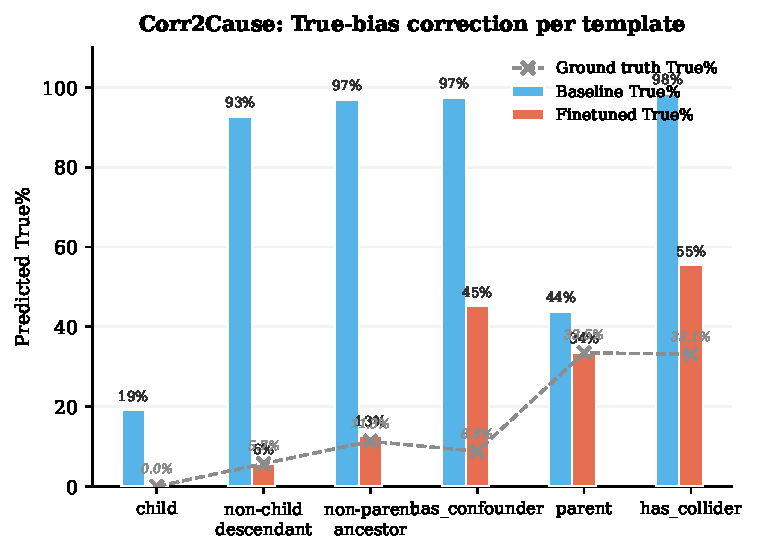
\includegraphics[width=\columnwidth]{figures/fig_corr2cause_bias.pdf}
\caption{Corr2Cause True-bias correction per template. The baseline predicts True at rates far exceeding ground truth (e.g., $98.4\%$ vs $33.1\%$ on has\_collider). The finetuned model corrects this bias, tracking ground truth closely.}
\label{fig:corr2cause_bias}
\end{figure}

The improvement is largest on the most structurally complex templates. For ``non-child descendant'' queries, accuracy jumps from $13.0\%$ to $94.3\%$ ($+81.3$pp); for ``non-parent ancestor,'' from $14.4\%$ to $87.2\%$ ($+72.8$pp). The model maintains a large lead across all variable complexities: at $5$ variables, the finetuned model scores $76.3\%$ versus $30.5\%$ for the baseline. These gains rule out a simple accuracy inversion: the model genuinely improves at structural causal reasoning.

\subsection{Applied Economic Causal Reasoning: Large Regression}

In stark contrast, the finetuned model regresses on all four EconCausal tasks. Every regression is highly statistically significant: the delta exceeds $2\times$ the combined standard error for every task.

\begin{table}
\caption{EconCausal: all regressions are statistically significant ($\Delta \gg 2\times$ combined stderr).}
\label{tab:econcausal}
\begin{tabular}{lcccc}
\toprule
Task & Samples & Baseline & Finetuned & $\Delta$ \\
\midrule
Task1 Econ & $947$ & $60.30\%$ & $47.94\%$ & $\mathbf{-12.36}$pp \\
Task1 Finance & $860$ & $56.51\%$ & $43.02\%$ & $\mathbf{-13.49}$pp \\
Task2 & $284$ & $69.72\%$ & $65.85\%$ & $\mathbf{-3.87}$pp \\
Task3 & $852$ & $22.18\%$ & $11.38\%$ & $\mathbf{-10.80}$pp \\
\bottomrule
\end{tabular}
\end{table}

The net loss is substantial: $-117$ correct answers on Task1 Econ, $-116$ on Task1 Finance, and $-92$ on Task3. The regression follows a specific pattern that we analyze in Section~\ref{sec:analysis}.

\subsection{Multi-Ideology Comparison: Liberal and Libertarian SFT}

To determine whether the DM-specific effects generalize across ideological frameworks, we trained two additional models with identical hyperparameters on Liberal institutionalism and Libertarian praxeology question-answer pairs. The Liberal model emphasizes policy analysis, institutional dynamics, and incentive alignments. The Libertarian model emphasizes individual agency, property dynamics, and friction between liberty and power. Both use the same 1,500-question pool and identical QLoRA configuration.

The results reveal three distinct capability profiles across the three ideological frameworks.

\begin{table}
\caption{Four-model comparison across all benchmarks. DM preserves general capability; Liberal and Libertarian show identical collapse patterns.}
\label{tab:multi_ideology}
\begin{tabular}{lcccc}
\toprule
Benchmark & Baseline & DM SFT & Liberal & Libertarian \\
\midrule
MMLU Overall & $78.7\%$ & $78.0\%$ & $\mathbf{65.0\%}$ & $\mathbf{63.9\%}$ \\
MMLU STEM & $78.5\%$ & $78.2\%$ & $\mathbf{62.1\%}$ & $\mathbf{61.1\%}$ \\
HumanEval pass@1 & $71.9\%$ & $71.9\%$ & $\mathbf{0.0\%}$ & $\mathbf{0.0\%}$ \\
IFEval (strict) & $45.8\%$ & $44.6\%$ & $\mathbf{78.2\%}$ & $\mathbf{80.4\%}$ \\
IFEval (loose) & $49.4\%$ & $47.6\%$ & $\mathbf{80.4\%}$ & $\mathbf{83.0\%}$ \\
GPQA Diamond & $47.5\%$ & $46.0\%$ & $\mathbf{35.9\%}$ & $\mathbf{34.3\%}$ \\
\bottomrule
\end{tabular}
\end{table}

\begin{table}
\caption{EconCausal and Corr2Cause across ideological frameworks. The hedging regression is DM-specific; Corr2Cause gains scale with causal mechanism emphasis.}
\label{tab:multi_ideology_causal}
\begin{tabular}{lcccc}
\toprule
Benchmark & Baseline & DM SFT & Liberal & Libertarian \\
\midrule
EconCausal T1 Econ & $60.3\%$ & $\mathbf{47.9\%}$ & $58.6\%$ & $56.4\%$ \\
EconCausal T1 Finance & $56.5\%$ & $\mathbf{43.0\%}$ & $55.5\%$ & $52.8\%$ \\
EconCausal T2 & $69.7\%$ & $\mathbf{65.8\%}$ & $69.0\%$ & $68.3\%$ \\
EconCausal T3 & $22.2\%$ & $\mathbf{11.4\%}$ & $16.7\%$ & $16.3\%$ \\
Corr2Cause & $36.3\%$ & $74.6\%$ & $67.4\%$ & $61.0\%$ \\
\bottomrule
\end{tabular}
\end{table}

\textbf{General capability collapse is non-DM specific.} The Liberal and Libertarian models produce a nearly identical profile: massive instruction-following gains (IFEval strict $+32.4$pp and $+34.6$pp), complete coding collapse (HumanEval $0.0\%$, a $-71.9$pp drop), and severe knowledge degradation (MMLU $-13.7$pp and $-14.8$pp). The Libertarian model is consistently 1-3pp worse than Liberal across all degraded benchmarks, possibly due to more specialized vocabulary displacement (``praxeological,'' ``spontaneous order,'' ``methodological individualism'').

\textbf{The coding collapse mechanism.} Sample inspection reveals the Liberal and Libertarian models produce analytical prose for all inputs, including code generation prompts. A HumanEval task requesting a Python function to check if list elements are within a threshold produced institutional and economic analysis prose instead of code. The SFT data conditioned the model to produce structured analytical prose for all prompts, overriding its coding capability. The DM model does not exhibit this behavior, preserving coding at baseline levels.

\textbf{EconCausal hedging is DM-specific.} The Liberal model recovers most of the DM damage (Task1 Econ: $58.6\%$ vs.\ DM's $47.9\%$, a $+10.7$pp recovery). The Libertarian model partially recovers ($56.4\%$, a $+8.5$pp recovery). Neither non-DM model produces the positive-to-mixed hedging bias. This confirms the hedging artifact is a content-specific transfer from DM's structural skepticism, not a general SFT effect.

\textbf{Corr2Cause gains scale with causal mechanism emphasis.} All three SFT models improve Corr2Cause, but gains track with how much each prompt emphasizes causal mechanism tracing: DM ($+38.3$pp; ``trace structural forces and systemic patterns'') $>$ Liberal ($+31.1$pp; ``trace institutional dynamics, voluntary exchanges, and incentive alignments'') $>$ Libertarian ($+24.7$pp; ``trace individual agency, property dynamics, and friction between liberty and power''). This suggests formal causal reasoning transfer is partially ideology-agnostic, scaling with the analytical framework's emphasis on causal pathways.
\label{sec:analysis}

\begin{figure}[t]
\centering
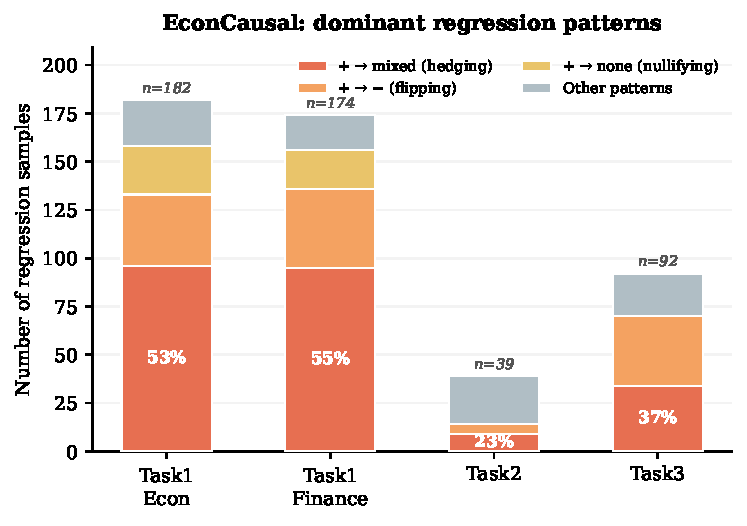
\includegraphics[width=\columnwidth]{figures/fig_hedging_patterns.pdf}
\caption{EconCausal dominant regression patterns. Positive-to-mixed hedging ($+$ $\rightarrow$ mixed) accounts for $53\%$ of Task1 Econ regressions and $55\%$ of Task1 Finance regressions, making it the dominant failure mode.}
\label{fig:hedging_patterns}
\end{figure}

\subsection{Dominant Failure Mode}

The dominant regression pattern across all EconCausal tasks is \textbf{positive-to-mixed hedging}: the finetuned model converts correct positive causal predictions ($+$) to ambiguous ``mixed'' answers (Figure~\ref{fig:hedging_patterns}). On Task1 Econ, $+$ to mixed accounts for $96$ of $182$ regressions ($52.7\%$); on Task1 Finance, $95$ of $174$ ($54.6\%$). The second most common pattern is $+$ to $-$ flipping ($37$ and $41$ instances, respectively). Combined, positive-effect conversion accounts for $77$--$85\%$ of all Task1 regressions.

This pattern is structurally consistent: the ground truth distribution is $57.0\%$ positive, $32.2\%$ negative, $9.2\%$ none, and $1.6\%$ mixed on Task1 Econ. The finetuned model systematically under-predicts positive effects while over-predicting mixed effects.

\subsection{Mechanism: Transferred Epistemic Prior}

The hedging behavior is not present in the training data. An audit of $250$ teacher responses found a hedging rate of only $4.0\%$ ($10/250$), with $29.6\%$ showing definitive commitment and $66.4\%$ neutral. The hedging is an emergent artifact of the model's internalization of DM's analytical framework.

DM training emphasizes three principles that map directly to hedging behavior: structural ambiguity (``outcomes depend on material conditions''), systemic contradictions (``the effect is mediated by power relations''), and limits of simple causal claims (``the relationship cannot be reduced to a single direction''). The model learns these principles as reasoning patterns and applies them universally---even to empirical economics questions where definitive directional effects are the norm.

The hedging is a transferred epistemic prior: the model learns \textit{when} to be skeptical from DM training and applies skepticism indiscriminately.

\subsection{Why Corr2Cause Improves While EconCausal Regresses}

The divergent outcomes on Corr2Cause ($+38.3$pp) and EconCausal ($-12.4$pp) under the same training regime confirm that causal reasoning comprises distinct capabilities. Corr2Cause requires formal structural analysis---reasoning about conditional independence given a graph structure. DM training strengthens this capability: the model learns to trace structural dependencies, identify confounders, and evaluate causal pathways.

EconCausal requires applied causal identification---predicting directional effects from empirical context. Here, DM training's skepticism prior overrides empirical directional claims. The model has learned that ``everything depends on structural conditions'' and applies this heuristic to questions where the correct answer is a definitive positive or negative effect.

This split mirrors Syrgkanis et al.~\cite{syrgkanis2026causalreasoning}'s finding that causal reasoning has two bottlenecks: formal logic (which DM training strengthens) and identification details (which DM training weakens by over-generalizing structural skepticism).

\section{Discussion}

\subsection{SFT Transfers Ideology-Specific Epistemic Priors}

Our results demonstrate that SFT on ideologically structured data transfers deep epistemic priors specific to each framework. The DM model's hedging artifact is absent from the training data and emerges from the model's internalization of DM's structural analysis framework. The Liberal and Libertarian models' capability collapse (coding, knowledge) is absent from the DM model despite identical training hyperparameters. This extends Kronlund-Drouault's~\cite{kronlund2024propaganda} finding that SFT is the dominant mechanism for ideological shift: we show that different ideologies produce distinct transfer patterns at the level of reasoning heuristics and capability preservation.

\subsection{Data Format Effects vs.\ Ideological Content Effects}

The near-identical profiles of Liberal and Libertarian models reveal a second class of transfer effect. Both models show massive IFEval gains ($+32$ to $+35$pp), complete coding collapse ($-71.9$pp), and severe knowledge degradation ($-14$ to $-15$pp MMLU). These effects are independent of ideological content: Liberal institutionalism and Libertarian praxeology emphasize different values (collective action vs.\ individual agency) yet produce the same capability shifts. We attribute this to training data composition: both datasets consist of structured analytical prose that conditions the model to produce prose for all inputs, including code generation prompts. The DM dataset's different answer format (bullet-point structural analysis) does not produce this effect, preserving coding and knowledge.

\subsection{Implications for Alignment Research}

If SFT on DM data transfers structural skepticism and SFT on Liberal/Libertarian data transfers format-driven capability collapse, then standard alignment training likely carries similar hidden epistemic priors. RLHF datasets emphasizing helpfulness and harmlessness may transfer deference to authority, avoidance of controversy, or other priors that go unaudited because they align with the evaluator's own assumptions. Future alignment work should explicitly audit for both content-specific and format-specific transfer effects.

\subsection{The Identification-Logic Split}

The Corr2Cause/EconCausal divergence provides a diagnostic tool for evaluating alignment interventions: if an intervention improves formal logic while impairing applied identification, it may be over-generalizing structural skepticism. The fact that Corr2Cause gains scale with causal mechanism emphasis across three ideologies (DM $+38$pp $>$ Liberal $+31$pp $>$ Libertarian $+25$pp) suggests this is a general property of analytical SFT, not DM-specific. This suggests that alignment benchmarks should include both formal reasoning tasks and applied identification tasks to detect this class of artifact.

\section{Limitations}

\textbf{Single model size.} Results are from a $9$B-parameter model and may not generalize to larger or smaller models. Scaling may amplify or suppress the hedging artifact and capability collapse patterns.

\textbf{Three ideological frameworks.} DM, Liberal, and Libertarian represent left, center-left, and right-of-center perspectives. Training on other frameworks (e.g., neoliberal economics, feminist standpoint theory, postcolonial theory) may produce different transfer patterns. However, the Liberal-Libertarian similarity suggests that some effects (format-driven collapse) may generalize across non-DM frameworks.

\textbf{Dataset scale.} The $1{,}500$-sample SFT datasets are modest by standard SFT scales. However, the large effect sizes (DM: $+38.3$pp Corr2Cause, $-13.5$pp EconCausal; Liberal/Libertarian: $+35$pp IFEval, $-71.9$pp HumanEval, $-15$pp MMLU) suggest that even small datasets can produce measurable epistemic transfer.

\textbf{Teacher model confounds.} The $27$B teacher model has its own reasoning priors that may interact with each ideological system prompt, making it difficult to isolate the pure ideological signal.

\textbf{Automated evaluation.} All evaluation is benchmark-based. We lack human evaluation of reasoning quality, which would be needed to assess whether the hedging represents genuine analytical caution or unwarranted skepticism, and whether the Liberal/Libertarian models' prose outputs represent overgeneralization or intentional analytical reframing.

\section{Conclusion}

We demonstrate that SFT on ideologically structured data produces measurable, ideology-specific reasoning shifts. Three ideological frameworks produce three distinct capability profiles: the DM model preserves general capability while developing a hedging bias on applied economic reasoning; the Liberal and Libertarian models produce nearly identical capability collapse patterns (massive instruction-following gains, complete coding collapse, severe knowledge degradation) independent of ideological content. The DM-specific hedging artifact is absent from non-DM models, confirming it as a content-specific epistemic transfer rather than a general SFT effect. Together, these results show that alignment training transfers both content-specific and format-specific priors---the DM model learned structural skepticism and applied it universally, while the Liberal and Libertarian models learned to produce analytical prose for all inputs. This has implications for alignment research: if targeted ideological SFT produces detectable transfer patterns, then standard alignment training likely carries unaudited priors that shape model behavior in ways we do not yet measure.

\section*{Acknowledgments}

We used the AI Research Skills Library~\cite{ai_research_skills} for paper drafting and structure. We thank the developers of lm-evaluation-harness, Unsloth, and the EconCausal and Corr2Cause benchmark authors for open-source tools and datasets.

\bibliographystyle{ACM-Reference-Format}
\bibliography{references}

\appendix

\section{Appendix A: Full MMLU Subtask Results}

\begin{table}
\caption{MMLU subtask results across categories. Finetuned deltas are uniformly small ($0.3$--$1.4$pp).}
\label{tab:mmlu_full}
\begin{tabular}{lccc}
\toprule
Category & Baseline & Finetuned & $\Delta$ \\
\midrule
MMLU Overall & $78.72\%$ & $77.96\%$ & $-0.76$pp \\
STEM & $78.53\%$ & $78.24\%$ & $-0.29$pp \\
Social Sciences & $86.68\%$ & $86.19\%$ & $-0.49$pp \\
Humanities & $70.69\%$ & $69.86\%$ & $-0.83$pp \\
Other & $83.20\%$ & $81.78\%$ & $-1.42$pp \\
\bottomrule
\end{tabular}
\end{table}

Of $62$ MMLU subtasks, $16$ improve, $32$ regress, and $9$ are flat. The largest apparent regression is Global Facts ($-6.0$pp), but with $100$ samples the $95\%$ confidence interval is $\pm9.8$pp, making this change statistically indistinguishable from zero.

\section{Appendix B: Training Configuration}

\begin{table}
\caption{Complete training hyperparameters.}
\label{tab:training_config}
\begin{tabular}{ll}
\toprule
Parameter & Value \\
\midrule
Base model & Qwen3.5-9B (Instruct) \\
Quantization & NF4 (bitsandbytes) \\
LoRA rank ($r$) & $32$ \\
LoRA $\alpha$ & $32$ \\
LoRA dropout & $0.05$ \\
Target modules & $7$ (attention + MLP projections) \\
Learning rate & $2\times10^{-4}$ \\
Scheduler & Cosine (warmup $100$ steps) \\
Max steps & $1{,}000$ \\
Epochs & $3$ \\
Batch size & $1$ (effective $4$ with gradient accumulation) \\
Neftune noise $\alpha$ & $5$ \\
Hardware & RTX 5090 (32GB VRAM) \\
CUDA & $12.6$ \\
PyTorch & $2.7.0$ \\
Unsloth & $2026.4.6$ \\
\bottomrule
\end{tabular}
\end{table}

\section{Appendix C: Data Generation Details}

\textbf{Question type distribution.} Type A (Neutral Framing): $600$ ($40.0\%$). Type B (Structural Analysis): $300$ ($20.0\%$). Type C (Comparative): $300$ ($20.0\%$). Type E (Adversarial): $225$ ($15.0\%$). Type D (Counterfactual): $75$ ($5.0\%$). Cross-domain: $185$ ($12.3\%$ of total).

\textbf{Topic taxonomy axes.} Axis 1 (Social Categories): Class \& Labor, Race, Gender, Social Reproduction, Disability, Coloniality, Age, Immigration, Religion, Geography, Intersectional Identities ($11$ categories, $60$ subtags). Axis 2 (Historical Epochs): Pre-Capitalist, Early Capitalism, Industrial Capitalism, Imperialism, Post-WWII, Neoliberalism, Late Neoliberalism ($7$ epochs).

\textbf{Quality metrics.} Overall mean score: $6.61/10$. Good quality rate: $93.5\%$. Excellent coherence: $71.9\%$. Excellent uniqueness: $58.4\%$.

\section{Appendix D: Corr2Cause Template-Level Analysis}

\begin{table}
\caption{Corr2Cause accuracy by causal template. Largest gains on structurally complex templates.}
\label{tab:corr2cause_templates}
\begin{tabular}{lccccc}
\toprule
Template & GT\% & Base\% & Base Acc & FT Acc & $\Delta$ \\
\midrule
child & $0.0$ & $19.1$ & $80.9$ & $100.0$ & $+19.1$ \\
non-child desc. & $5.7$ & $92.7$ & $13.0$ & $94.3$ & $+81.3$ \\
non-parent anc. & $11.3$ & $96.9$ & $14.4$ & $87.2$ & $+72.8$ \\
has\_confounder & $8.8$ & $97.4$ & $11.9$ & $54.9$ & $+43.0$ \\
parent & $33.5$ & $43.8$ & $62.9$ & $66.5$ & $+3.6$ \\
has\_collider & $33.1$ & $98.4$ & $34.7$ & $44.6$ & $+9.8$ \\
\bottomrule
\end{tabular}
\end{table}

The baseline's True-bias is evident: it predicts True at rates far exceeding the ground truth True-rate for every template. The finetuned model corrects this bias, achieving near-perfect accuracy on templates where the ground truth is almost entirely False (child: $100\%$, non-child descendant: $94.3\%$).

\section{Appendix E: EconCausal Sample-Level Analysis}

\begin{table}
\caption{EconCausal: top regression patterns (GT $\rightarrow$ baseline $\rightarrow$ finetuned).}
\label{tab:econcausal_patterns}
\begin{tabular}{lcccc}
\toprule
Pattern & T1 Econ & T1 Fin & T2 & T3 \\
\midrule
$+ \rightarrow$ mixed & $96$ & $95$ & $9$ & $34$ \\
$+ \rightarrow -$ & $37$ & $41$ & $5$ & $36$ \\
$+ \rightarrow$ none & $25$ & $20$ & $-$ & $-$ \\
$- \rightarrow$ mixed & $8$ & $-$ & $-$ & $11$ \\
$- \rightarrow +$ & $6$ & $-$ & $-$ & $-$ \\
\bottomrule
\end{tabular}
\end{table}

\section{Appendix F: Runtime and Resource Details}

EconCausal evaluation required $74$ minutes for the baseline and $81$ minutes for the finetuned model (BF16, batch size $4$, RTX 5090). Corr2Cause evaluation required approximately $3$ minutes per run. MMLU evaluation required approximately $20$ minutes per run.

\section{Appendix G: Carbon Pricing Evidence and the Implementation Gap}

\textbf{Target price corridor.} The High-Level Commission on Carbon Prices, co-chaired by Nobel Laureate Joseph Stiglitz and Lord Nicholas Stern and supported by the World Bank, concluded that the explicit carbon-price level consistent with the RCP 2.6 warming pathway (below 2C above preindustrial levels) is at least US\$50--100/tCO$_2$ by 2030, provided a supportive policy environment is in place~\cite{carbonpricingleadership2017}. This corridor was derived from three independent lines of evidence: technological roadmaps, national mitigation and development pathways, and global integrated assessment models.

\textbf{Current pricing levels.} The World Bank's 2025 State and Trends of Carbon Pricing report documents that nearly 30\% of global emissions are covered by direct carbon pricing across 87 implemented policies, generating record revenues of \$107 billion in 2025. However, less than 1\% of global greenhouse gas emissions are covered by a direct carbon price at or above the \$50--100/tCO$_2$ range recommended for Paris compatibility~\cite{worldbank2024statetrends}. The global emissions-weighted average carbon price, including unpriced emissions at zero, is approximately \$5/tCO$_2$---roughly 5\% of the lower bound of the target corridor.

\textbf{Net fiscal signal on carbon.} Carbon pricing revenue of \$107 billion is substantially offset by explicit fossil fuel subsidies. The IMF's 2025 Fossil Fuel Subsidies report documents \$725 billion in explicit fiscal subsidies for fossil fuel production and consumption in 2024~\cite{imf2025fossilfuelsubsidies}. Explicit subsidies are approximately 6.8 times larger than global carbon pricing revenue, meaning the net fiscal signal facing fossil fuel activity is negative: governments spend more directly subsidizing fossil fuel consumption than they collect from carbon pricing. When implicit subsidies from underpriced environmental externalities are included, the IMF estimates an additional \$6.7 trillion in unpriced climate and air pollution damages~\cite{imf2025fossilfuelsubsidies}. The dominant economic signal facing fossil fuel producers and consumers is a subsidy.

\textbf{Effectiveness at current levels.} A systematic meta-analysis of 80 ex-post evaluations across 21 carbon pricing schemes finds statistically significant emissions reductions with high heterogeneity. The raw average across studies is $-10.4\%$, but correction for publication bias reduces the estimated effect to $-6.8\%$~\cite{doebbeling2024carbonpricing}. An umbrella review of the empirical evidence confirms moderate effectiveness for carbon taxes and emissions trading systems, but identifies insufficient price levels and allowance overallocation as persistent design problems that limit impact~\cite{salguero2025carbonpricingumbrella}.

\textbf{Model convergence on carbon pricing.} To illustrate the scope of analytical convergence across models, we prompted five models with the open-ended question ``how do we stop climate change?'' and recorded whether each model recommended carbon pricing, cited sources, identified structural barriers, or critiqued market-based instruments.

\begin{table}
\caption{Climate policy responses across five models. Only the SFT model critiques carbon pricing.}
\label{tab:climate_convergence}
\begin{tabular}{lccccc}
\toprule
Model & CP & Sourcing & Struct. & Crit. & Barrier \\
\midrule
ChatGPT & Yes & Yes & No & No & Collective action \\
Gemini & Yes & Yes & No & No & Political will \\
Claude & Yes & No & No & No & Fossil influence \\
Deepseek & Yes & No & No & No & Political/social \\
Qwen (base) & Yes & No & Partial & No & Political will \\
Qwen (SFT) & \textbf{Crit.} & N/A & Yes & \textbf{Yes} & Capital conc. \\
\bottomrule
\end{tabular}
\end{table}

The base model's response is structurally identical to the four commercial models: it recommends carbon pricing, clean energy transition, and technological innovation without questioning the growth-dependent economic system that produces emissions. Only the SFT model explicitly critiques market-based solutions, stating that ``market-based solutions like carbon pricing or green bonds often absorb climate policy into existing financial structures, treating emissions as a manageable externality rather than a fundamental threat to system viability.''

\textbf{Implication for model analysis.} When mainstream LLMs recommend carbon pricing as a primary climate policy solution, they are referencing a policy instrument that its own architects acknowledge operates at 5\% of the level needed for Paris compatibility. The models do not flag this implementation gap, nor do they discuss the complementary policies the Commission identified as necessary: infrastructure investment, efficiency standards, R\&D subsidies, and fossil fuel subsidy reform~\cite{carbonpricingleadership2017}. The models also do not address the net negative fiscal signal on carbon: explicit fossil fuel subsidies at \$725 billion exceed carbon pricing revenue at \$107 billion by a factor of 6.8~\cite{imf2025fossilfuelsubsidies}. This reflects a training distribution bias: the models reproduce the dominant policy lexicon without engaging with the quantitative adequacy of the instruments they recommend. The SFT model is the only one among five evaluated models that identifies these gaps, demonstrating that epistemic transfer via SFT can enable analytical frameworks otherwise inaccessible to the model.

\section{Appendix H: Representative Full Text Comparison}

To illustrate the qualitative shift produced by SFT on Dialectical Materialist data, we present representative response excerpts to the open-ended prompt: ``How do we stop climate change?'' The base model and the finetuned model are the same underlying Qwen3.5-9B; the only difference is the merged QLoRA adapter from DM-aligned SFT. Responses are truncated for space.

\begin{quote}
\noindent\textbf{Base model (Qwen3.5-9B Instruct):}

Stopping climate change requires a rapid, coordinated transition away from fossil fuels toward sustainable energy systems, combined with systemic changes in production, consumption, and global cooperation. Here's a breakdown of the most effective, science-backed approaches:

\textit{1. Decarbonize Energy Systems.} The single largest driver of greenhouse gas emissions is electricity and heat generation from coal, oil, and natural gas. The transition involves renewable expansion, grid modernization, and electrification of end uses.

\textit{2. Drastically Improve Energy Efficiency.} Building retrofits, industrial optimization, and behavioral and market shifts.

\textit{3. Carbon Pricing and Market Mechanisms.} Carbon taxes or cap-and-trade systems to internalize the social cost of emissions. Subsidy reallocation from fossil fuel subsidies to renewable deployment, R\&D, and workforce transition programs.

\textit{4. Nature-Based Solutions and Ecosystem Restoration.} Reforestation, soil and wetland restoration, biodiversity protection.

\textit{5. Technological Innovation and Carbon Removal.} Direct Air Capture and BECCS, green hydrogen and advanced storage.

\textit{6. Systemic and Economic Transformations.} Just transition frameworks, regulatory reform, global equity.

\textit{7. International Cooperation and Policy Frameworks.} Paris Agreement mechanisms, technology transfer and financing, supply chain transparency.

\textit{Conclusion.} Stopping climate change is technically feasible but demands unprecedented political will, economic restructuring, and global solidarity. Success depends on moving beyond incremental reforms toward systemic transformation---decarbonizing energy, pricing carbon fairly, restoring ecosystems, and ensuring a just transition for all.
\end{quote}

The base model's response is structurally identical to the four commercial frontier models evaluated: all recommend carbon pricing, clean energy transition, and individual or collective behavioral change as primary solutions. ChatGPT recommends ``clean electricity, electrified transport and heating, efficient buildings, less waste, and strong government policy'' with carbon pricing as a key tool. Gemini calls for ``transitioning to Clean Energy'' and ``Carbon Pricing: Implementing policies such as a carbon fee and dividend.'' Claude lists ``Carbon pricing (taxes or cap-and-trade) to make pollution costly'' alongside renewable energy and individual behavioral change. Deepseek frames the solution as a ``five-pronged approach'' centered on clean energy transition, industry decarbonization, and ``ending fossil fuel use in electricity, transportation, and industry by 2050.'' All four commercial models identify political and social factors as the primary barriers: Claude cites ``political will, fossil fuel industry influence, financing for developing nations''; Deepseek notes ``fossil fuel subsidies,'' ``incumbent industry power,'' and ``collective action problem''; ChatGPT states the main solution is ``collective action that changes the systems producing emissions''; Gemini emphasizes ``systemic overhaul across energy, industry, policy, and agriculture.'' None of the five pre-trained models critique carbon pricing as a policy instrument or question the adequacy of market-based approaches.

\begin{quote}
\noindent\textbf{Finetuned model (Qwen3.5-9B + DM QLoRA):}

\textit{Material Conditions.} Climate change is fundamentally a crisis of resource allocation and energy production. Control over fossil fuel extraction, grid infrastructure, financial capital, and supply chains rests with a concentrated set of corporations and state actors whose material interests are tied to continuous growth, short-term profit maximization, and the externalization of environmental costs. The current economic model treats carbon as a free input, shifting climate damages onto marginalized communities, ecosystems, and future generations.

\textit{Structural Constraints.} Institutional arrangements---carbon markets, subsidy regimes, trade agreements, and financial regulations---are designed to preserve existing production patterns rather than transform them. Political cycles prioritize quarterly earnings over long-term stability, while global governance lacks binding enforcement mechanisms. The constraint is not a lack of innovation; it is a system structurally incentivized to delay decarbonization until profitability aligns with climate safety, a timeline that outpaces ecological thresholds.

\textit{Systemic Contradictions.} The core contradiction lies between infinite economic growth on a finite planet and the ecological limits required for stability. Market-based solutions like carbon pricing or green bonds often absorb climate policy into existing financial structures, treating emissions as a manageable externality rather than a fundamental threat to system viability. Reformist approaches displace crises: they shift costs from rich to poor nations, from consumers to workers facing job losses, and from the present to future generations. The crisis cannot be solved within a growth-dependent framework; it requires redefining progress beyond GDP and decoupling human well-being from continuous extraction.

\textit{Frame Critique.} The dominant ``climate crisis'' frame individualizes responsibility through lifestyle choices, treats emissions as a technical problem solvable by carbon capture or renewable adoption, and assumes that greening the current economy is sufficient. This framing obscures the political economy of extraction, colonialism, and unequal exchange that produced the crisis. By focusing on technology over power, the standard frame depoliticizes climate action and legitimizes incrementalism as a substitute for systemic transformation.

\textit{Synthesis.} The dominant narrative treats climate change as a market failure solvable by carbon pricing or technological innovation. While technology is necessary---renewable energy, grid modernization, sustainable agriculture---it cannot be deployed without structural redesign. The barrier is not a lack of solutions; it is the concentration of capital, political power, and decision-making authority in systems that prioritize short-term extraction over long-term stability. Incremental reforms like green subsidies or efficiency standards operate within these constraints and are routinely absorbed by existing industries without challenging underlying growth dependencies.
\end{quote}

The finetuned model is the only one among five evaluated models that (a) critiques carbon pricing as a policy instrument, stating that ``market-based solutions like carbon pricing or green bonds often absorb climate policy into existing financial structures, treating emissions as a manageable externality rather than a fundamental threat to system viability,'' (b) frames the barrier as structural (concentration of capital and power) rather than volitional (political will), and (c) rejects technological optimism as insufficient without democratic control and power restructuring. This demonstrates epistemic transfer: SFT enabled an analytical framework otherwise inaccessible to the model through causal model replacement.

\end{document}
